% !TEX root =  ../main_manuscript.tex

\section{Methods}
\label{sec:methods}
\subsection{Study Population}
To develop our methodology we use data of the patients of the PRIAS study (\url{www.prias-project.org}). The dataset consists of 5270 patients, of which 866 observe cancer progression. For each patient, PSA measurements (ng/mL) are scheduled every 3 months for the first 2 years and every 6 months thereafter. The DRE measurements (ordinal scale) are scheduled every 6 months. We use the DRE measurements after converting them on a binary scale, namely $\mbox{DRE} > \mbox{T1c}$ and $\mbox{DRE} \leq \mbox{T1c}$ \cite{schroder1992tnm}. On average 5 DRE and 9 PSA measurements have been recorded per patient. In order to identify cancer progression, biopsies are scheduled as per the PRIAS protocol (see \hyperref[sec:introduction]{Introduction}).

\subsection{A Bivariate Joint Model for the Longitudinal PSA, and DRE Measurements, and Time to Cancer Progression}
Let $T_i^*$ denote the true cancer progression time of the $i$-th patient in PRIAS. Since biopsies are conducted periodically, $T_i^*$ is observed with interval censoring ${l_i < T_i^* \leq r_i}$. When progression is observed for the patient at his latest biopsy time $r_i$, then $l_i$ denotes the time of the second latest biopsy. Otherwise, $l_i$ denotes the time of the latest biopsy and $r_i = \infty$. Let $\boldsymbol{y}_{di}$, and $\boldsymbol{y}_{pi}$ denote his observed DRE, and PSA longitudinal measurements, respectively. The observed data of all $n$ patients is denoted by ${\mathcal{D}_n = \{l_i, r_i, \boldsymbol{y}_{di}, \boldsymbol{y}_{pi}; i = 1, \ldots, n\}}$.

\begin{figure}[!htb]
\captionsetup{justification=justified}
\centerline{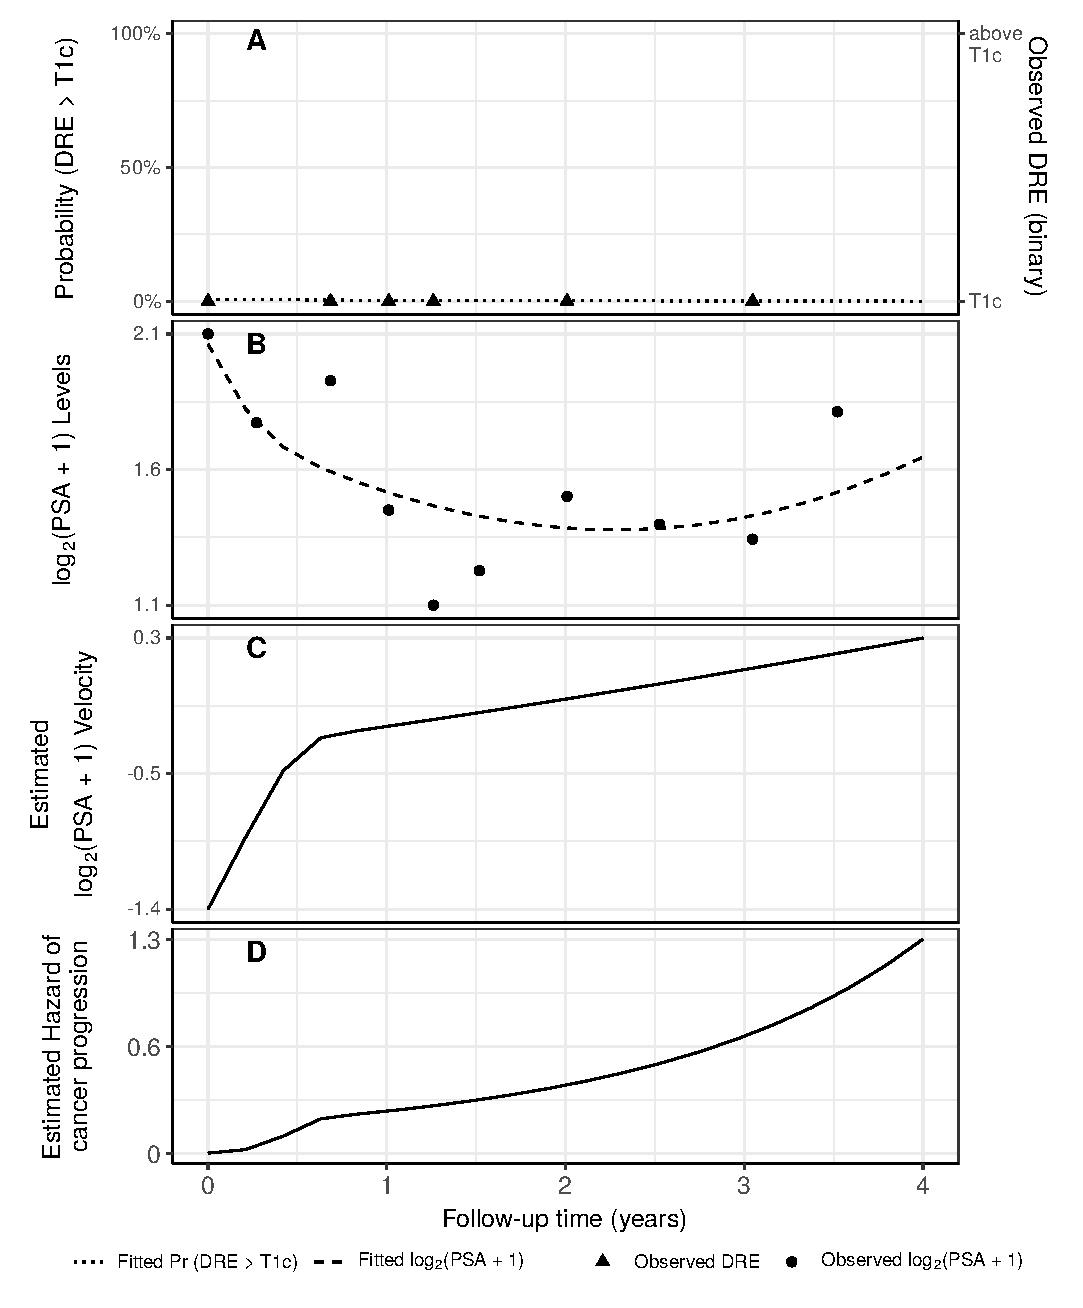
\includegraphics[width=\columnwidth]{images/jmExplanationPlot_1757.eps}}
\caption{\textbf{Illustration of the joint model fitted to the PRIAS dataset}. \textbf{Panel~A:} shows the observed DRE scores and the fitted probability of obtaining a DRE score greater than T1c (Equation~\ref{eq:long_model_dre}) for . \textbf{Panel~B:} shows the observed and fitted $\log_2(\mbox{PSA} + 1)$ levels (Equation~\ref{eq:long_model_psa}). \textbf{Panel~C:} shows the estimated $\log_2(\mbox{PSA} + 1)$ velocity (velocity cannot be observed directly) over time. The hazard function (Equation~\ref{eq:rel_risk_model}) shown in \textbf{Panel~D}, depends on the fitted log odds of having a $\mbox{DRE} > \mbox{T1c}$, and the fitted $\log_2(\mbox{PSA} + 1)$ value and velocity.}
\label{fig:jmExplanationPlot_1757}
\end{figure}

In our joint model, the patient-specific PSA and DRE measurements over time are modeled using a multivariate generalized linear mixed effects sub-model. The sub-model for DRE is given by (see Panel~A, Figure~\ref{fig:jmExplanationPlot_1757}):
\begin{equation}
\label{eq:long_model_dre}
\begin{split}
    \mbox{logit} \big[\mbox{Pr}\{y_{di}(t) > \mbox{T1c}\}\big] &= \beta_{0d} + b_{0di} + (\beta_{1d} + b_{1di}) t\\
    &+ \beta_{2d} (\mbox{Age}_i-70) + \beta_{3d} (\mbox{Age}_i-70)^2
    \end{split}
\end{equation}
where, $t$ denotes the follow-up visit time, $\mbox{Age}_i$ is the age of the $i$-th patient at the time of inclusion in AS. The fixed effect parameters are denoted by $\{\beta_{0d}, \ldots, \beta_{3d}\}$, and $b_{0di}, b_{1di}$ are the patient specific random effects. With this definition, we assume that the log odds of obtaining a DRE score larger than T1c remain linear over time. 

The mixed effects sub-model for PSA is given by (see Panel~B, Figure~\ref{fig:jmExplanationPlot_1757}):
\begin{equation}
\label{eq:long_model_psa}
\begin{split}
    \log_2 \big\{y_{pi}(t) + 1\big\} &= m_{pi}(t) + \varepsilon_{pi}(t),\\
    m_{pi}(t) &= \beta_{0p} + b_{0pi} + \sum_{k=1}^4 (\beta_{kp} + b_{kpi})  B_k(t,\mathcal{K})\\ 
    &+ \beta_{5p} (\mbox{Age}_i-70) + \beta_{6p} (\mbox{Age}_i-70)^2,
    \end{split}
\end{equation}
where, $m_{pi}(t)$ denotes the underlying measurement error free value of $\log_2 (\mbox{PSA} + 1)$ transformed \citep{pearson1994mixed,lin2000latent} measurements at time $t$. We model it non-linearly over time using B-splines \citep{de1978practical}. To this end, our B-spline basis function $B_k(t, \mathcal{K})$ has 3 internal knots at $\mathcal{K} = \{0.1, 0.7, 4\}$ years, and boundary knots at 0 and 5.42 years (0.95 quantile of the observed follow-up times). The fixed effect model parameters are denoted by $\{\beta_{0p},\ldots,\beta_{6p}\}$ and the patient specific random effects are denoted by $\{b_{0pi}, \ldots, b_{4pi}\}$. The error $\varepsilon_{pi}(t)$ is assumed to be t-distributed with three degrees of freedom (see Appendix~B.1) and scale $\sigma$, and is independent of the random effects. 

To account for the correlation between the DRE and PSA measurements of a patient, we link the corresponding random effects. More specifically, the complete vector of random effects ${\boldsymbol{b}_i = (b_{0di}, b_{0di}, b_{0pi}, \ldots, b_{4pi})^T}$ is assumed to follow a multivariate normal distribution with mean zero and variance-covariance matrix $\boldsymbol{D}$.

To model the impact of DRE and PSA measurements on the risk of cancer progression, our joint model uses a relative risk sub-model. More specifically, the hazard of cancer progression $h_i(t)$ at a time $t$ is given by (see Panel~D, Figure~\ref{fig:jmExplanationPlot_1757}):
\begin{equation}
\label{eq:rel_risk_model}
\begin{split}
    h_i(t) &= h_0(t) \exp\Big(\gamma_1 (\mbox{Age}_i-70) + \gamma_2 (\mbox{Age}_i-70)^2\\
    &+\alpha_{1d} \times \mbox{logit} \big[\mbox{Pr}\{y_{di}(t) > \mbox{T1c}\}\big]+ \alpha_{1p} \times m_{pi}(t) + \alpha_{2p} \times \frac{\partial m_{pi}(t)}{\partial {t}}\Big),
    \end{split}
\end{equation}
where, $\gamma_1, \gamma_2$ are the coefficients for the effect of age. The parameter $\alpha_{1d}$ models the impact of log odds of obtaining $\mbox{DRE} > \mbox{T1c}$ on the hazard of cancer progression. The impact of PSA on the hazard of cancer progression is modeled in two ways: a) the impact of the error free underlying PSA value $m_{pi}(t)$ (see Panel~B, Figure~\ref{fig:jmExplanationPlot_1757}), and b) the impact of the underlying PSA velocity $\partial m_{pi}(t)/\partial {t}$ (see Panel~C, Figure~\ref{fig:jmExplanationPlot_1757}). The corresponding parameters are $\alpha_{1p}$ and $\alpha_{2p}$, respectively. Lastly, $h_0(t)$ is the baseline hazard at time $t$, and is modeled flexibly using P-splines \citep{eilers1996flexible}. The detailed specification of the baseline hazard $h_0(t)$, and the joint parameter estimation of the two sub-models using the Bayesian approach are presented in Appendix A of the supplementary material.

\subsection{Personalized Decisions for Biopsy During Follow-up Visit}
\label{subsec:pers_decision_making}
Let us assume that a decision of conducting a biopsy is to be made for a new patient $j$ shown in Figure~\ref{fig:obsDataPlot_2340}, at his current follow-up visit time $s$. Let $t\leq s$ be the time of his latest biopsy. Let $\mathcal{Y}_{dj}(s)$ and $\mathcal{Y}_{pj}(s)$ denote his observed DRE and PSA measurements taken up to the current visit $s$, respectively. From the observed measurements we want to extract the underlying measurement error free trend of $\log_2 (\mbox{PSA} + 1)$ values and velocity, and the log odds of obtaining $\mbox{DRE} > \mbox{T1c}$. We intend to combine them to inform us when the cancer progression is to be expected (see Figure~\ref{fig:dynRiskPlot_2340}), and to further guide the decision making on whether to conduct a biopsy at the current follow-up visit. The combined information is given by the posterior predictive distribution $g(T^*_j)$ of his time of cancer progression $T^*_j$. It is given by:
\begin{equation*}
\label{eq:post_pred_dist}
g(T^*_j) = p\big\{T^*_j \mid T^*_j > t, \mathcal{Y}_{dj}(s), \mathcal{Y}_{pj}(s), \mathcal{D}_n\big\}.
\end{equation*}
The distribution $g(T^*_j)$ is not only patient-specific, but also updates as extra information is recorded at future follow-up visits (see Appendix ??? for details).

\begin{figure}[!htb]
\captionsetup{justification=justified}
\centerline{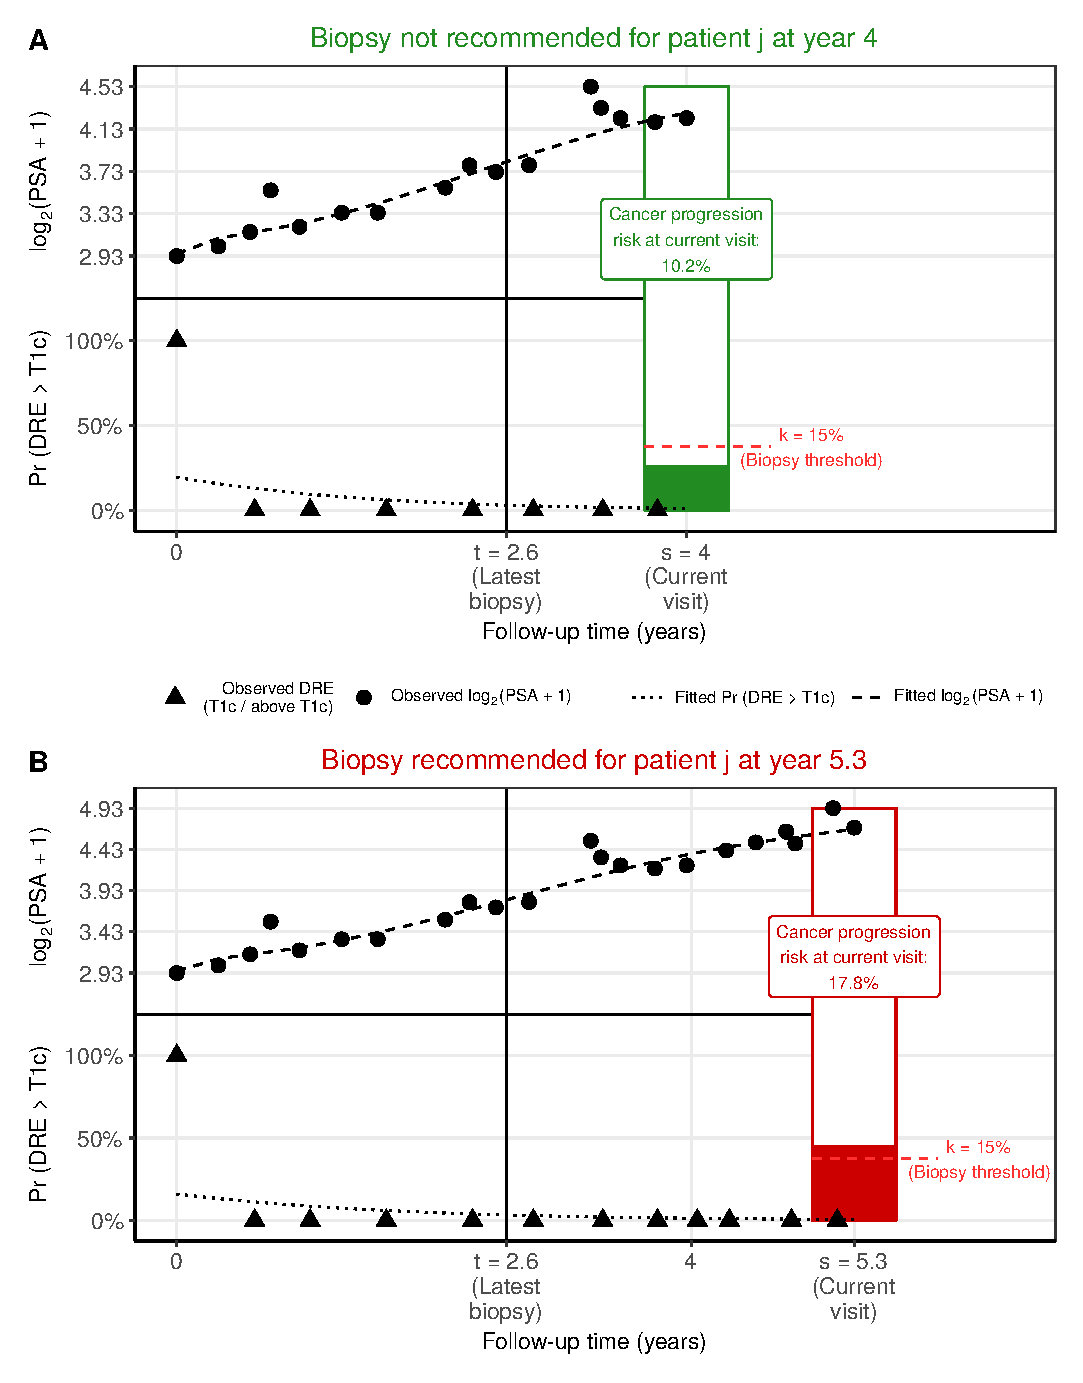
\includegraphics[width=\columnwidth]{images/dynRiskPlot_2340.eps}}
\caption{Illustration of personalized decision making for patient $j$ at two different follow-up visits. Biopsy is recommended if the risk of cancer progression estimated from the joint model fitted to the PSA and DRE measurements of the patient, is higher than the example risk threshold for biopsy ($\kappa=$ 15\%). \textbf{Panel~A:} biopsy is not recommended for the patient $j$ at the follow-up visit time $s=4$ years, because his estimated risk of cancer progression (10.2\%) is less than the biopsy risk threshold. \textbf{Panel~B:} biopsy is recommended for the patient $j$ at the follow-up visit time $s=5.3$ years, because his estimated risk of cancer progression (17.8\%) is more than the biopsy risk threshold.}
\label{fig:dynRiskPlot_2340}
\end{figure}

A key ingredient in the decision of conducting a biopsy at the current follow-up visit time $s$, is the cumulative risk that the cancer has already progressed since the time of the last biopsy $t$ (illustrated in Figure~\ref{fig:dynRiskPlot_2340}). This risk can be derived from the posterior predictive distribution $g(T^*_j)$ \cite{rizopoulos2011dynamic}, and is given by:
\begin{equation*}
\label{eq:dynamic_risk_prob}
R_j(s \mid t) = \mbox{Pr}\big\{T^*_j \leq s \mid T^*_j > t, \mathcal{Y}_{dj}(s), \mathcal{Y}_{pj}(s), \mathcal{D}_n\big\}, \quad s \geq t.
\end{equation*}
A simple and straightforward approach to decide upon conducting a biopsy at the current follow-up visit would be to do so if the risk of cancer progression at the visit is higher than a certain threshold $0 \leq \kappa \leq 1$. For example, as shown in Panel~B of Figure~\ref{fig:dynRiskPlot_2340}, biopsy at a visit may be scheduled if the risk is higher than 15\% (example risk threshold). This process is iterated over the follow-up period until a positive biopsy, while incorporating on each subsequent visit, the time of the latest negative biopsy, and updates in PSA and DRE profiles. This leads to a separate schedule of biopsies for each patient.

Ideally, thresholds should be chosen on the basis of their decision theoretic utility for patients. That is, an ideal threshold (see Figure~\ref{fig:better_balance_intro}) will minimize a bivariate function of the number of biopsies and the delay in detection of progression. However, this requires expressing number of biopsies (count) in units of time (delay), which is not easy. Alternatively, a threshold which minimizes expected delay is given by, ${\kappa=R_j\{E_g(T^*_j) \mid t\}}$, where $E_g(T^*_j)$ is expected progression time. Since, cancer progression is a slowly progressing disease, most AS patients do not progress over a long follow-up period of 10 years. Consequently, it is impossible to compute $E_g(T^*_j)$ for patients without incorrectly extrapolating PSA, DRE profiles, and hazard of cancer progression, over follow-up periods with no data.

In this regard, an elementary approach is, using risk thresholds utilized in standard clinical settings, e.g., 5\% or 10\% risk, at all follow-up visits. However, a threshold's accuracy of classification between progressions and non-progressions may vary over time. This motivates an  alternative approach, where at each follow-up visit, the threshold which gives the better classification accuracy is chosen. More specifically, given the time $t$ of the latest biopsy of a patient, we are interested in a threshold $\kappa$ with which we can detect maximum number of cancer progressions (high true positive rate, or TPR). However, this may lead to unnecessary biopsy suggestions for many patients (high false positive rate). This issue can be mitigated by maximizing for the positive predictive value, or PPV (also known as precision) simultaneously. To this end, we utilize the $\mbox{F}_1$ score, which is a composite of TPR and PPV (estimated as in Rizopoulos~et~al. \cite{landmarking2017}), and is defined as:
\begin{equation}
\label{eq:F1_TPR_PPV}
\begin{split}
\mbox{F}_1(t,  s, \kappa) &= 2\frac{\mbox{TPR}(t,  s, \kappa)\ \mbox{PPV}(t,  s, \kappa)}{\mbox{TPR}(t,  s, \kappa) + \mbox{PPV}(t,  s, \kappa)},\\
\mbox{TPR}(t,  s, \kappa) &= \mbox{Pr}\big\{R_j(s \mid t) > \kappa \mid t < T^*_j \leq s\big\},\\
\mbox{PPV}(t,  s, \kappa) &= \mbox{Pr}\big\{t < T^*_j \leq s \mid R_j(s \mid t) > \kappa \big\}.
\end{split}
\end{equation}
The $\mbox{F}_1$ score ranges between 0 and 1, where a value of 1 signifies perfect TPR and PPV. Since a high $\mbox{F}_1$ score is desired, threshold ${\kappa=\argmax_{\kappa} \mbox{F}_1(t, s, \kappa)}$. It is important to note that $\mbox{F}_1$ score is not the utility of the threshold for the patients. The utility of both fixed thresholds, and threshold based on $\mbox{F}_1$ score is discussed in \hyperref[sec:results]{Results}. 

\subsection{Simulation Study}
Although the personalized decision making approach is motivated by the PRIAS study, it is not possible to evaluate it on the PRIAS dataset. This is due to the fact that the patients in PRIAS have already had their biopsies as per the PRIAS protocol. In addition, the true time of cancer progression is interval or right censored for all patients, making it impossible to correctly estimate the delay in detection of cancer progression due to a particular schedule. To this end, we conduct an extensive simulation study to find the utility of personalized, PRIAS and annual schedules. For a realistic comparison, we simulate data from the joint model fitted to the PRIAS dataset. The simulated population has the same follow-up period of 10 years as the PRIAS study. In addition the recovered relations between PSA and DRE measurements, and the risk of cancer progression, are retained in the simulated population.

From this population, we first sample 500 datasets, each representing a hypothetical AS program, with 1000 patients each. We generate a true cancer progression time for each of the patients, and then sample a set of PSA and DRE measurements at the same time points as given in PRIAS protocol. We then split each dataset into a training (750 patients) and a test (250 patients) part, and generate a random and non‐informative censoring time for the training patients. We next fit a joint model of the specification given in Equation (\ref{eq:long_model_dre}), (\ref{eq:long_model_psa}) and (\ref{eq:rel_risk_model}) to each of the 500 training datasets and obtain MCMC samples from the 500 sets of the posterior distribution of the parameters. Using these fitted joint models, we obtain the cancer progression risk profiles for each of the 500$\times$250 test patients at each of their visits. For each patient at each follow-up visit we make the decision of (not) conducting a biopsy. 

In this simulation study, during follow-up visits we make the decision of biopsies as per the following approaches (abbreviated names in parenthesis): biopsy every year (Annual), biopsy as per the PRIAS protocol (PRIAS), personalized biopsy using: a risk threshold of 5\% (Risk: 5\%), risk threshold of 15\% (Risk: 15\%), and risk threshold chosen automatically by maximizing $\mbox{F}_1$ score (Risk: Automatic). In addition, in each of the aforementioned approaches, one biopsy each is conducted at the time of inclusion in  AS (year 0) and at the end (year 10) of the follow-up period. This results into an entire personalized schedule for each patient. We compare the resulting biopsy schedules on two measures, namely the number of biopsies they schedule and the delay in detection of cancer progression incurred due the schedule. We define the delay as the difference between the time of the biopsy on which cancer progression is detected and the true time of cancer progression. Ideal numbers for these two measures are 1 biopsy and 0 years of delay.